\documentclass[unicode,a4paper,12pt,russian,openany]{book}
\usepackage{cmap}
\usepackage[left=1.5cm,right=1.5cm,
    top=1.5cm,bottom=1.5cm,bindingoffset=0cm]{geometry}
\usepackage[dvips]{graphicx}
\usepackage[unicode=true]{hyperref}
\usepackage[cm-default]{fontspec}
\usepackage{xunicode}
\usepackage{xltxtra}
\usepackage{polyglossia}
\usepackage{wrapfig}
\usepackage{listings}
\usepackage{color}
\usepackage{xcolor,mdframed}
\usepackage{subfigure}
\usepackage{textcomp}
\definecolor{dkgreen}{rgb}{0,0.6,0}
\definecolor{mauve}{rgb}{0.58,0,0.82} 
\lstset{ %
  language=bash,
  backgroundcolor=\color{white},
  frame=single,
  rulecolor=\color{black},
  tabsize=2,
  breaklines=true,
  breakatwhitespace=true, 
  keywordstyle=\color{blue},
  commentstyle=\color{dkgreen},
  stringstyle=\color{mauve} 
}
\newenvironment{important}[1][]{%
   \begin{mdframed}[%
      backgroundcolor={red!15}, hidealllines=true,
      skipabove=0.7\baselineskip, skipbelow=0.7\baselineskip,
      splitbottomskip=2pt, splittopskip=4pt, #1]%
   \makebox[0pt]{% ignore the withd of !
      \smash{% ignor the height of !
         \fontsize{32pt}{32pt}\selectfont% make the ! bigger
         \hspace*{-19pt}% move ! to the left
         \raisebox{-2pt}{% move ! up a little
            {\color{red!70!black}\sffamily\bfseries !}% type the bold red !
         }%
      }%
   }%
}{\end{mdframed}}
\defaultfontfeatures{Mapping=tex-text}
\setmainfont{Liberation Serif}
\newfontfamily\cyrillicfont{Liberation Serif}
\setmonofont{Liberation Mono}
\newfontfamily\cyrillicfonttt{Liberation Mono}
\setsansfont{Liberation Sans}
\newfontfamily\cyrillicfont{Liberation Sans}
\setdefaultlanguage[spelling=modern]{russian}
\setotherlanguage{english}
\setcounter{tocdepth}{3}
\graphicspath{{images/}}
\begin{document}

\begin{titlepage}

\begin{center}
Работа анонимного исследователя
\vspace{10em}

\rule{\linewidth}{0.5mm}
\LARGE \textbf{Настольная книга анонима}\\
\Large \textbf{Зачем нужна анонимность и как её достичь?}
\rule{\linewidth}{0.5mm}
\vfill
\normalsize Растространяется на условиях Creative Commons Zero 1.0\\
\url{http://creativecommons.org/publicdomain/zero/1.0}\\
\begin{figure}[h]
\center{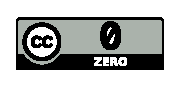
\includegraphics[width=0.15\linewidth]{cc-zero}}
\end{figure}
2012 год
\end{center}

\end{titlepage}


\tableofcontents

\chapter*{Введение}
\addcontentsline{toc}{part}{Введение}
\section{Причины появления книги}
В последнее время правительства многих стран стремятся уничтожить анонимность, оправдываясь <<безопасностью граждан>>. Однако данное стремление направлено не на увеличение безопасности, оно направлено только на усиление контроля. Чиновникам нужна уверенность в том, что на следующий день они не потеряют своего кресла, что вы пролосуете за них на следующих выборах, что вы не узнаете об их лжи, что вы не выйдете на улицы, недовольные их произволом, что они продолжат также воровать деньги из бюджета и брать взятки. Они ищут способ контроля. Государства, называющие себя демократическими, становятся авторитарными. Но правительства, вмешивающиеся в личную жизнь, не являются единственной причиной жажды анонимности. За вами может также следить ваш работодатель, хозяин хот-спота в любимой кафешке, администрация вашего учебного заведения. Маркетологи следят за вами, чтобы показать вам более таргетированную рекламу. Организации, борющиеся с пиратством, следят за вами, чтобы отсудить у вас деньги за две скачаненые композиции уже умершего певца. И если вас все это не устраивает, то данная книга для вас.

\section{Связь с автором}
Вы можете сообщить об ошибках или связаться со мной по иным причинам с помощью электронной почты \href{mailto:anonhandbook@tormail.org}{anonhandbook@tormail.org} или отправив свои изменения в репозиторий \url{https://gitorious.org/anonymous-handbook}.
\part{Необходимость анонимности в современном мире}
\chapter{Политические причины}
\section{Журналисты}
С 1993 по 2009 год в России было убито 176 журналистов\cite{kill}.
\subsection{Избиение Михаила Бекетова}
\subsection{Нападение на Олега Кашина}
\subsection{Избиение Константина Фетисова}
\subsection{Убийство Анны Политковской}
\subsection{Убийство Натальи Эстемировой}
\subsection{Убийство Магомеда Евлоева}
\section{Гражданские активисты}
\chapter{Нетехнические методы}
\section{Нераскрытие информации}
Чтобы сохранить анонимность вы, как ни странно, не должны сами не раскрывать лишнюю информацию. Информация об одном лишь поле позволяет сократить число вариантов примерно в два раза. Комбинируя известную информацию, легко можно определить конкретного человека. Не распространяйтесь ни о своем роде занятий, ни о музыкальных вкусах, ни тем более о месте жительства и возрасте, если хотите остаться анонимным. Избегайте лишних вопросов.
\section{Ложная информация}
Для того, чтобы воспрепятствовать процессу установления вашей реальной личности вы можете специально давать ложную информацию. Например, вы можете сказать, что вы из Саратова, живя в Ростове-на-Дону. Поскольку тот, кто хочет установить вашу личность, не знает, где правда, а где ложь, то ваша ложь сильно усложняет ему задачу. Придумайте виртуального персонажа с выдуманными данными, от имени которого вы будете выступать.
\section{Лингвистический анализ}
Даже если вы не указываете в тексте личной информации, остается возможным установление вашей личности. Допущенные в тексте ошибки, сленг или редкоиспользуемые слова и многая другая информация, добытая лингвистическим анализом, может помочь в установлении личности автора. При составлении текстов, авторство которых вы хотите сохранить в секрете, используйте стиль, отличный от стиля, которым вы пользуетесь в реальной жизни.

\chapter{Технические методы}
\begin{important}
Не стоит забывать, что следующие методы необходимо использовать, по возможности, совместно друг с другом и с методами, перечисленными в предыдущей главе.
\end{important}
\section{Прокси}

\section{VPN}

\section{SSH-туннели}

\section{Настойка браузера Firefox}
\subsection{Подмена информации, передаваемой браузером}
\begin{important}
Браузер передает огромное количество информации. По отдельности эта информация не представляет никакого интереса, но собранная вместе она может позволить практически со 100\% вероятностью установить вашу личность.
\end{important}
\subsubsection{User-agent}
\subsubsection{Часовой пояс}
\subsubsection{Предпочитаемые языки}
\subsection{Дополнения}
\subsubsection{HTTPS Everywhere}
\subsubsection{BetterPrivacy}
\subsubsection{Ghostery}
\subsubsection{TrackerBlock}
\subsubsection{Beef Taco}
\subsubsection{User Agent Changer}

\section{Анонимные оверлейные сети}
\textbf{Оверлейные сети} --- это такие сети, которые работают поверх другой уже работающей сети.
\subsection{Tor}
\begin{wrapfigure}[9]{r}{0.25\linewidth}

\includegraphics[width=\linewidth]{Tor}
\caption{Логотип Tor}
\end{wrapfigure}
\textbf{Tor} --- анонимная оверлейная сеть, использующая принцип луковой маршрутизации, исходные коды которой распространяются на условиях лицензии BSD\cite{tor_license}.\\
\textbf{Луковая маршрутизация} --- технология анонимного обмена информацией, использующая многократное шифрование и пересылку через цепочки узлов. Каждый луковый маршрутизатор в цепочке удаляет слой шифрования и пересылает сообщение дальше, согласно полученным инструкциям, где все повторится. И так до тех пор, пока сообщение не достигнет адресата. Такое название технология получила из-за сходства данного процесса с очисткой луковицы.\\
\subsubsection{Установка}
\subsubsection{Использование}
\subsubsection{Недостатки}
\begin{important}
Не забывайте, что при использовании обычного Интернета через Tor, последняя нода в цепочке (exit-нода) видит трафик нешифрованным.
\end{important}
\subsection{I2P}
\begin{wrapfigure}[6]{r}{0.25\linewidth}
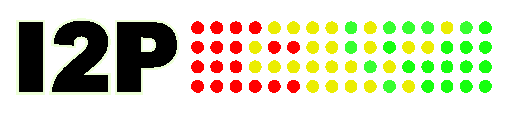
\includegraphics[width=\linewidth]{I2P}
\caption{Логотип I2P}
\end{wrapfigure}
\textbf{I2P} --- анонимная оверлейная сеть, использующая принцип чесночной маршрутизации, исходные коды которой распространяются на условиях нескольких свободных лицензий\cite{i2p_license}. В отличии от Tor, который в первую очередь направлен на доступ к сайтам обычного интернета (хотя в нем и существуют скрытые сервисы, аналогичные ипсайтам в I2P, а в I2P можно получить доступ к внешнему Интернету, используя аутпрокси), основной целью I2P является доступ именно к скрытым ресурсам --- ипсайтам. Ипсайт от обычного вебсайта отличает только его нахождение в сети I2P.\\
\textbf{Чесночная маршрутизация} --- вариант луковой, отличающийся тем, что несколько <<луковиц>> пересылаются совместно, что усложняет установку авторства сообщений.
\subsubsection{Установка}
\subsubsection{Использование}
\subsubsection{Недостатки}
\subsection{Freenet}
\begin{wrapfigure}[9]{r}{0.25\linewidth}

\includegraphics[width=\linewidth]{Freenet}
\caption{Логотип Freenet}
\end{wrapfigure}
\textbf{Freenet} --- анонимная оверлейная сеть, использующая принципы P2P и F2F и распространяющаяся на условиях GNU GPL v2\cite{freenet_license}. В отличии от Tor и I2P, позволяющих размещать любые ресурсы внутри сети, Freenet по сути представляет собой хранилище статичных данных.\\
\textbf{P2P (Peer-to-peer)} --- компьютерная сеть, в которой все участники равны и выполняют одновременно роль как клиента, так и сервера.\\
\textbf{F2F (Friend-to-Friend)} --- разновидность P2P-сети, в которой все соединения разрешаются только с доверенными узлами.
\subsubsection{Установка}
\subsubsection{Использование}
\subsubsection{Недостатки}

\section{Анонимные платежи}
\subsection{Анонимные пластиковые карточки}
\subsection{Bitcoin}
\subsection{Прочие платежные системы}

\section{IM-сервисы}
\subsection{I2P-Messenger}
\subsection{TorChat}
\subsection{Cryptocat}

\section{Ремейлеры}
\subsection{Типы ремейлеров}
\subsection{Mixmaster}
\subsection{Mixminion}

\section{Прием почты}
\subsection{I2P-Mail}
\subsection{I2P-Bote}
\subsection{TorMail}
\subsection{Privacybox}

\section{Шифрование данных}
\subsection{Truecrypt}
\subsection{dm-crypt}
\subsection{GPG}

\section{Шифрование передаваемой информации}
\subsection{Off-the-Record Messaging (OTR)}
\subsection{GPG и Jabber}
\subsection{GPG м любая другая передаваемая информация}

\section{Стеганография}
\textbf{Стеганография} --- способ тайной передачи информации путем сохранения в тайне самого факта передачи информации. Чаще всего используется совместно с криптографическими методами.

\subsection{steghide}
\begin{figure}[ht!]
\vspace{-4ex}
\centering
\subfigure[]{
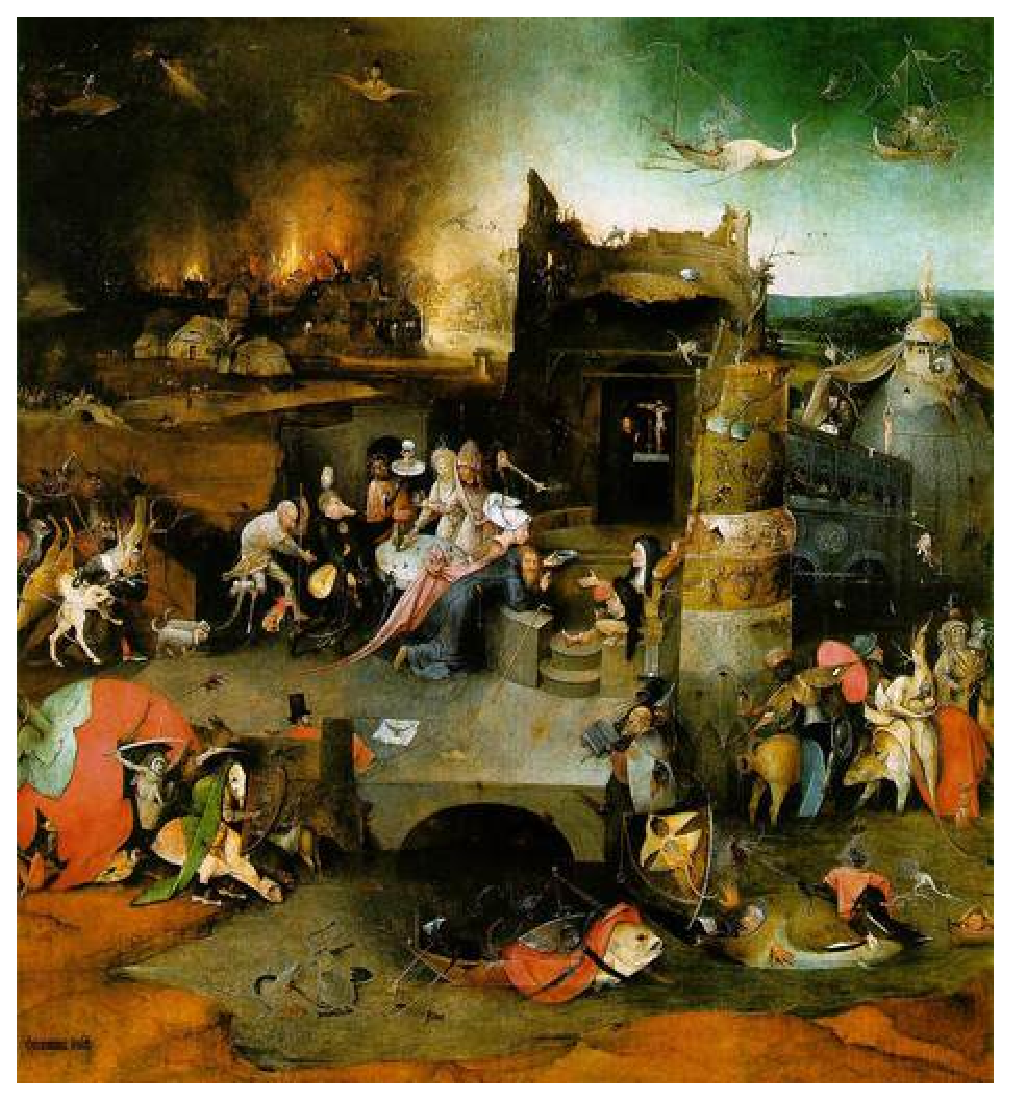
\includegraphics[width=0.25\linewidth]{steghide1}
\label{fig:steghide1}
}
\hspace{4ex}
\subfigure[]{
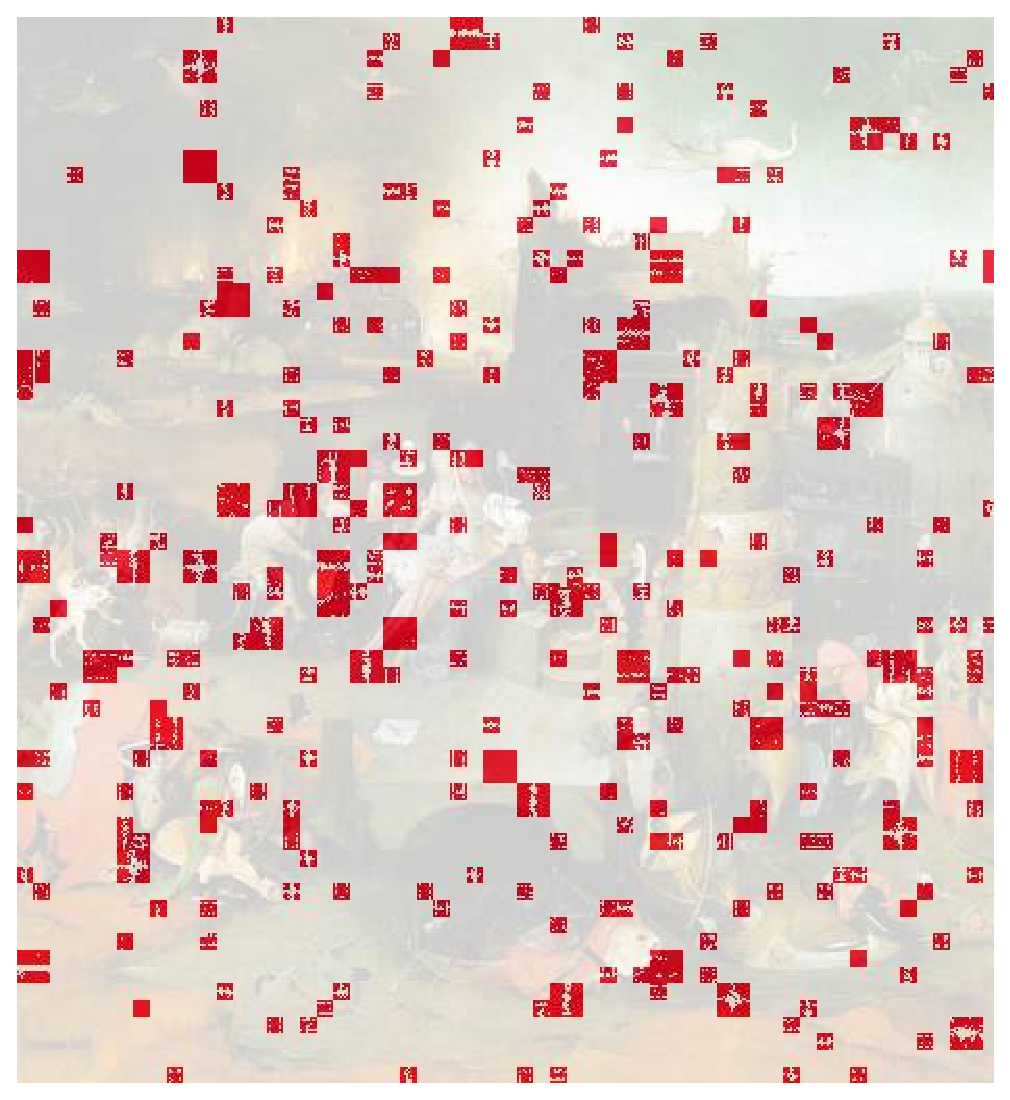
\includegraphics[width=0.25\linewidth]{steghide2}
\label{fig:steghide2}
}
\hspace{4ex}
\subfigure[]{
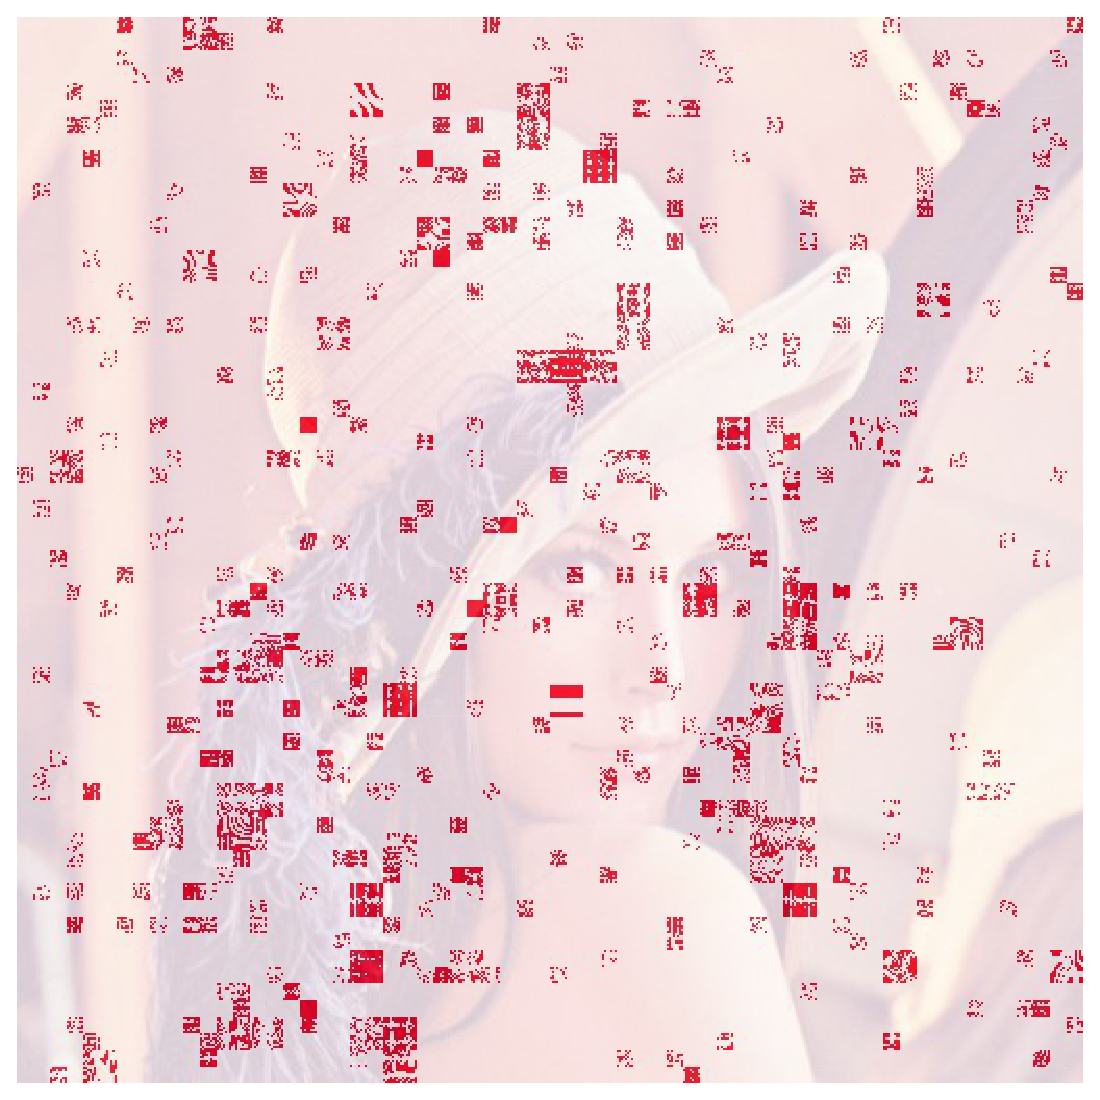
\includegraphics[width=0.25\linewidth]{steghide3}
\label{fig:steghide3}
}
\caption{Использование steghide: 
\subref{fig:steghide1} исходное изображение; 
\subref{fig:steghide2} в изображении закодирована фраза <<Feci quod potui, faciant meliora potentes>> с паролем <<cogitoergosum>>; 
\subref{fig:steghide3}} разница между изображениями.
\end{figure}
\subsubsection{Установка}
\subsubsection{Использование}
Вставка данных в изображение:
\begin{lstlisting}
steghide embed -cf "coverfile.jpg" -ef "embedfile.txt" -sf "stegofile.jpg" -p "password"
\end{lstlisting}
coverfile.jpg --- файл, в который вставляются данные.\\
embedfile.txt --- файл, который вставляется в изображение.\\
stegofile.jpg --- файл со вставленным изображением.\\
password --- пароль.\\\\
Извлечение данных:
\begin{lstlisting}
steghide extract -sf "stegofile.jpg" -p "password" -xf "extractfile.txt"
\end{lstlisting}
stegofile.jpg --- файл со вставленным изображением.\\
password --- пароль.\\
extractfile.txt --- файл, в который нужно записать извлеченные данные.
\subsubsection{Недостатки}
\newpage
\subsection{OpenStego}
\begin{figure}[h]
\center{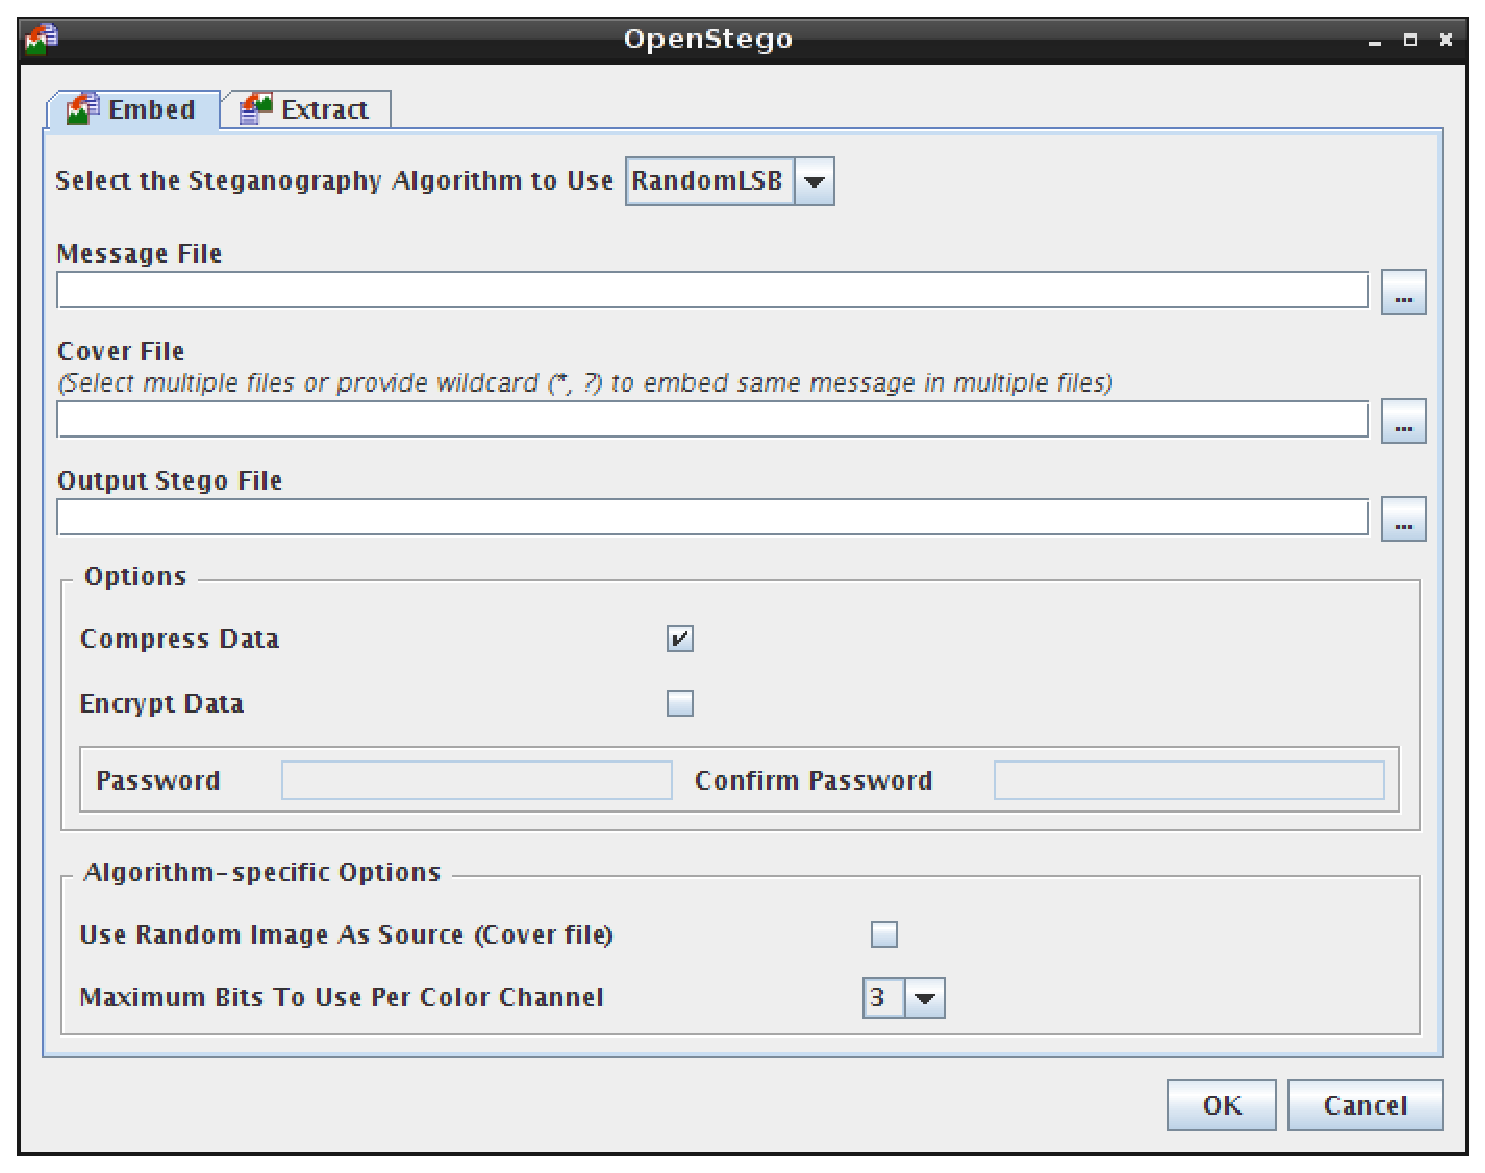
\includegraphics[width=0.75\linewidth]{openstego}}
\caption{Интерфейс OpenStego}
\end{figure}
\subsection{Желтые точки}
\begin{wrapfigure}[9]{r}{0.25\linewidth}
\includegraphics[width=\linewidth]{dots}
\caption{Желтые точки. Изображение: Parhamr}
\end{wrapfigure}
При печати материалов (например, листовок) не стоит забывать, что многие принтеры кодируют микроточками информацию о времени печати и о серийном номере принтера \cite{eff_dots}. Данная информация может быть использована для установления личности авторов отпечатков. Список принтеров, размещающих и не размещающих желтые точки смотрите в отчете Electronic Frontier Foundation\cite{eff_list}.

\section{Альтернативные DNS}
\subsection{Namecoin}
\subsection{OpenNIC}
\subsection{Собственный кеширующий DNS сервер}

\chapter{Дистрибутивы Linux}
\section{Debian}
\section{Ubuntu}
\section{Arch}
\section{Liberté Linux}
\chapter{Почему софт должен быть открытым?}
\section{Что такое OpenSource}
\section{Случаи}
\subsection{Обновление Windows с отключенной службой Windows Update}
\subsection{CarrierIQ}
\subsection{Возможность получить IP адрес любого пользователя Skype}
\chapter{Законы, гарантирующие свободу слова и анонимность}
\section{Статья 23 Конституции РФ}
\begin{enumerate}
\item Каждый имеет право на неприкосновенность частной жизни, личную и семейную тайну, защиту своей чести и доброго имени.
\item Каждый имеет право на тайну переписки, телефонных переговоров, почтовых, телеграфных и иных сообщений. Ограничение этого права допускается только на основании судебного решения.
\end{enumerate}
\section{Статья 24 Конституции РФ}
\begin{enumerate}
\item Сбор, хранение, использование и распространение информации о частной жизни лица без его согласия не допускаются.
\item Органы государственной власти и органы местного самоуправления, их должностные лица обязаны обеспечить каждому возможность ознакомления с документами и материалами, непосредственно затрагивающими его права и свободы, если иное не предусмотрено законом.
\end{enumerate}
\section{Статья 29 Конституции РФ}
\begin{enumerate}
\item Каждому гарантируется свобода мысли и слова.
\item Не допускаются пропаганда или агитация, возбуждающие социальную, расовую, национальную или религиозную ненависть и вражду. Запрещается пропаганда социального, расового, национального, религиозного или языкового превосходства.
\item Никто не может быть принужден к выражению своих мнений и убеждений или отказу от них.
\item Каждый имеет право свободно искать, получать, передавать, производить и распространять информацию любым законным способом. Перечень сведений, составляющих государственную тайну, определяется федеральным законом.
\item Гарантируется свобода массовой информации. Цензура запрещается.
\end{enumerate}
\chapter{Законы, гарантирующие свободу слова и анонимность}
\section{Статья 23 Конституции РФ}
\begin{enumerate}
\item Каждый имеет право на неприкосновенность частной жизни, личную и семейную тайну, защиту своей чести и доброго имени.
\item Каждый имеет право на тайну переписки, телефонных переговоров, почтовых, телеграфных и иных сообщений. Ограничение этого права допускается только на основании судебного решения.
\end{enumerate}
\section{Статья 24 Конституции РФ}
\begin{enumerate}
\item Сбор, хранение, использование и распространение информации о частной жизни лица без его согласия не допускаются.
\item Органы государственной власти и органы местного самоуправления, их должностные лица обязаны обеспечить каждому возможность ознакомления с документами и материалами, непосредственно затрагивающими его права и свободы, если иное не предусмотрено законом.
\end{enumerate}
\section{Статья 29 Конституции РФ}
\begin{enumerate}
\item Каждому гарантируется свобода мысли и слова.
\item Не допускаются пропаганда или агитация, возбуждающие социальную, расовую, национальную или религиозную ненависть и вражду. Запрещается пропаганда социального, расового, национального, религиозного или языкового превосходства.
\item Никто не может быть принужден к выражению своих мнений и убеждений или отказу от них.
\item Каждый имеет право свободно искать, получать, передавать, производить и распространять информацию любым законным способом. Перечень сведений, составляющих государственную тайну, определяется федеральным законом.
\item Гарантируется свобода массовой информации. Цензура запрещается.
\end{enumerate}
\chapter{Дальнейшее чтение}
\begin{enumerate}
\item 
\end{enumerate}


\newpage
\bibliographystyle{gost2008}
\bibliography{bibliography}

\end{document}
